
%%%%%%%%% MASTER -- compiles the 4 sections

%\documentclass[12pt,letterpaper]{article}
\documentclass[12pt,letterpaper,headings=normal]{scrartcl}

%%%%%%%%%%%%%%%%%%%%%%%%%%%%%%%%%%%%%%%%%%%%%%%%%%%%%%%%%%%%%%%%%%%%%%%%%
\pagestyle{plain}                                                      %%
%%%%%%%%%% EXACT 1in MARGINS %%%%%%%                                   %%
\setlength{\textwidth}{6.5in}     %%                                   %%
\setlength{\oddsidemargin}{0in}   %% (It is recommended that you       %%
\setlength{\evensidemargin}{0in}  %%  not change these parameters,     %%
\setlength{\textheight}{8.5in}    %%  at the risk of having your       %%
\setlength{\topmargin}{-.3in}       %%  proposal dismissed on the basis  %%
\setlength{\headheight}{0in}      %%  of incorrect formatting!!!)      %%
\setlength{\headsep}{0in}         %%                                   %%
\setlength{\footskip}{.2in}       %%                                   %%
%%%%%%%%%%%%%%%%%%%%%%%%%%%%%%%%%%%%                                   %%
\newcommand{\required}[1]{\section*{\hfil #1\hfil}}                    %%
\renewcommand{\refname}{\hfil References Cited\hfil}                   %%
\bibliographystyle{plain}                                              %%
%%%%%%%%%%%%%%%%%%%%%%%%%%%%%%%%%%%%%%%%%%%%%%%%%%%%%%%%%%%%%%%%%%%%%%%%%

%\setlength{\textheight}{9.4in}
%\renewcommand{\topfraction}{1}		% max fraction of floats at top
%\renewcommand{\bottomfraction}{1}	% max fraction of floats at bottom
%\def\overheader{-0.1in}
%\def\underheader{-0.1in}

\renewcommand{\rmdefault}{ptm} % Palatino=ppl or Times=ptm
\renewcommand{\sfdefault}{phv} % Helvetica
\renewcommand{\ttdefault}{pcr}  % Courier

\renewcommand{\thesection}{\Alph{section}} % change section nunbering to alphabetic

%PUT YOUR MACROS HERE
\usepackage{comment}
\usepackage{subfigure}
\usepackage{graphicx}
\usepackage{wrapfig}
\usepackage{url}
\usepackage{multicol}
\usepackage[margin=0pt,font=small,labelfont=bf,format=plain]{caption}
\usepackage{fancyhdr}
\usepackage{datetime}
\pagestyle{fancy}
\fancyhf{}
\renewcommand{\headrulewidth}{0pt}
\fancyhead[R]{\vspace{-1.5cm} \textit{Page =}~\thepage}
\usepackage{pdfpages}
\includepdfset{pagecommand=\thispagestyle{fancy}}
\usepackage{epsfig}


\begin{document}

%\markboth{\Large \bf Revised handout}{ }

%\baselineskip=24pt  % Enforce double space

\baselineskip=48pt  % Enforce double space

%\baselineskip=18pt  % Enforce 1.5 space
%
%\setlength{\parskip}{.3in}
%\setlength{\itemsep}{.3in}

\pagestyle{plain}

\vspace*{7cm}


\begin{center}
{\Large 
Rob 501 Handouts \\
Linear Algebra and Geometry
\mbox{ } \\
J.W. Grizzle \\
\mbox{ } \\
\mbox{ }
}
%{\bf Compiled on~\today~~at~\currenttime}
\end{center}



\newpage
\vspace*{10cm}
{\Large 
\begin{center}
Linear Algebra by Gabriel Nagy\\
\mbox{ } \\
 You can download the full textbook at the link given on the next page. We have permission to use it.  Professor Nagy warns us that there are some typos. \\
 \mbox{ }\\
 In the following, I have extracted 3 important chapters.
\end{center}
}
\newpage

\textbf{Sources:}
{\footnotesize
\begin{itemize}
\item Linear Algebra\\
\url{http://math.msu.edu/~gnagy/teaching/la.pdf}
\end{itemize}
}
%\newpage
%\vspace*{\fill}
%Chapter 4
\includepdf[pages=114-142]{BookChapters/LinearAlgebra/Nagy_LinearAlgebra_MichiganState.pdf}
%\vspace*{\fill}
%Chapter 6
\includepdf[pages=182-222]{BookChapters/LinearAlgebra/Nagy_LinearAlgebra_MichiganState.pdf}
%\vspace*{\fill}
%Chapter 7
\includepdf[pages=223-250]{BookChapters/LinearAlgebra/Nagy_LinearAlgebra_MichiganState.pdf}

\end{document}
